
\documentclass{article}

\usepackage[preprint, nonatbib]{neurips_2023}
\usepackage[utf8]{inputenc} % allow utf-8 input
\usepackage[T1]{fontenc}    % use 8-bit T1 fonts
\usepackage{hyperref}       % hyperlinks
\usepackage{url}            % simple URL typesetting
\usepackage{booktabs}       % professional-quality tables
\usepackage{amsfonts}       % blackboard math symbols
\usepackage{nicefrac}       % compact symbols for 1/2, etc.
\usepackage{microtype}      % microtypography
\usepackage{xcolor}         % colors
\usepackage{graphicx}       % images
\usepackage{subcaption}
\usepackage{enumitem}
% customized lists
\usepackage[backend=biber, style=ieee, url=false]{biblatex}
\addbibresource{ref.bib}


\newcommand{\todo}[1]{\fbox{\textcolor{red}{\bfseries #1} }}%
\newcommand{\figref}[1]{Figure \ref{#1}}
\newcommand{\tabref}[1]{Table \ref{#1}}


\title{Generating Volatility Surfaces of Index Options Using Variational Autoencoders (VAE)\\
\begin{large}
COS 513 -- Spring 2025 -- Project Proposal
\end{large} }

\author{%
Zhuolin Xiang \quad Haoqian Zhang \quad Siqing Zou\\
Princeton University \\
\texttt{\{zx4614,hz0531,sz6982\}@princeton.edu}
% Zhuolin Xiang\\
% Princeton University \\
% \texttt{zx4614@princeton.edu} \\
% \and
% Haoqian Zhang \\
% Princeton University \\
% \texttt{zhanghq.chn@gmail.com} \\
% \and
% Siqing Zou \\
% Princeton University \\
% \texttt{sz6982@princeton.edu} \\
}

\date{Week of February 3, 2025}

\begin{document}

\maketitle
% \begin{abstract}
%     Our project aims to explore the application of Variational Autoencoders (VAEs) in modeling and fitting the implied volatility surface of SPX index options. Traditional parametric models of stochastic volatility such as Heston and SABR impose rigid structural assumptions that may not fully capture market nuances. A VAE-based approach offers a flexible, data-driven alternative that can adapt to diverse market conditions, interpolate missing volatility data, and provide a generative framework for synthetic volatility surfaces. Our project will investigate the accuracy, robustness, and computational efficiency of VAEs compared to traditional models, with the goal of improving volatility estimation in options pricing and risk management.
% \end{abstract}

\section{Background and Motivations}


Volatility modeling is crucial in financial markets, as it underpins option pricing, risk management, and trading strategies. The implied volatility surface, which represents the market's expectations of future volatility across different strike prices and maturities, is fundamental to these applications. However, existing modeling methodologies have limitations. Parametric models like Heston and SABR rely on specific assumptions that may not generalize well across varying market conditions. Moreover, market-implied volatilities often contain missing or noisy data, requiring robust interpolation and extrapolation techniques. Given the advancements in generative models, methods like VAEs and LDMs provide a compelling alternative by learning a structured, low-dimensional representation of volatility surfaces without explicit assumptions about their shape.\\

Our project seeks to evaluate how VAEs can enhance volatility modeling by capturing latent structures and improving both interpolation and extrapolation capabilities. Additionally, we aim to analyze how these latent structures reflect underlying market conditions, providing deeper insights into volatility dynamics. Furthermore, we will explore the integration of VAEs with diffusion models, specifically Latent Diffusion Models (LDMs), to assess whether this hybrid approach can generate a more accurate and stable volatility surface. Code for this project is uploaded to our \href{https://github.com/zhanghq-chn/VAE-VolSurface.git}{Github repository}.

\section{Methodologies}
\paragraph{Variational Autoencoder (VAE)}
Our project will employ a VAE framework(see \figref{fig:a}) to model the SPX implied volatility surface. The VAE will be trained with an encoder-decoder structure, where the encoder maps the volatility surface into a latent space distribution, and the decoder reconstructs the surface from sampled latent variables. The training objective will balance reconstruction loss and Kullback-Leibler (KL) divergence to enforce meaningful latent representations. We follow the structure in \cite{vaeorigin} to construct the VAEs in two ways: the \textbf{grid-based} approach and the \textbf{pointwise} approach(see \figref{fig:b}).

\paragraph{Latent Diffusion Models (LDMs)}
To further enhance the performance, we will adopt a hybrid approach. LDMs in \cite{rombach2022highresolutionimagesynthesislatent} apply diffusion-based denoising techniques in the latent space rather than directly on high-dimensional volatility data, so we expect LDMs can  improve the quality of generated surfaces(i.e., robust extrapolation, reduced) while maintaining computational efficiency. Performance comparisons will be conducted to assess whether LDM-enhanced VAEs provide a superior alternative to standalone VAE and traditional parametric methods.



\paragraph{Evaluation} Once trained, the performance of our model will be evaluated through reconstruction error, interpolation accuracy, and generalization ability across different market conditions. The model’s output will be benchmarked against traditional stochastic models like Heston \cite{wolfram_volsurface_heston} and SABR \cite{wolfram_volsurface_sabr} to assess its viability as an alternative approach.

\section{Data}
\paragraph{Source} We initially focus on SPX option price data from 20220831 to 20230831 (We plan to include more data if it's required by the model training process). The data is available from  Wharton Research Data Services (WRDS). Key features include implied volatility, strike price, expiration date, best bid and best offer, etc.
\paragraph{Statistics} Since the original dataset consists of some extremely low liquidity options and some missing values, we conduct a cleaning process by keeping data with positive bid price, spread, open interest, and volume. We also filtered out extremely deep ITM and OTM options (whose absolute value of delta is not within 1\% and 99\% quantile). The summary statistics are exhibited in \tabref{tab:sm_stats}. One thing to note is that we have more put data than call, and the put data is more OTM. Additionally, we pick up 4 options with the highest trading volume and plot their volatility surface in \figref{fig:vol_surface}.


\begin{table}[h]
    \centering
    \textbf{Panel A: Call Options}
    \resizebox{\textwidth}{!}{\begin{tabular}{lrrrrrrrr}
\toprule
 & TTM & Moneyness & Spread & IV & Delta & Gamma & Vega & Theta \\
\midrule
Mean & 77.33 & 4235.42 & 6.37 & 0.19 & 0.38 & 0.00 & 413.03 & -435.17 \\
Median & 32.00 & 4190.00 & 1.59 & 0.18 & 0.35 & 0.00 & 313.22 & -334.64 \\
Min & 1.00 & 100.00 & 0.00 & 0.03 & 0.00 & 0.00 & 0.12 & -8681.90 \\
Max & 2002.00 & 12000.00 & 184.00 & 8.92 & 1.00 & 0.02 & 3782.84 & 110.52 \\
Std & 135.23 & 462.82 & 15.53 & 0.09 & 0.29 & 0.00 & 387.07 & 470.41 \\
Size & 644979.00 & 644979.00 & 644979.00 & 644979.00 & 644979.00 & 644979.00 & 644979.00 & 644979.00 \\
\bottomrule
\end{tabular}

}
    \vspace{5pt}

    \textbf{Panel B: Put Options}
    \resizebox{\textwidth}{!}{\begin{tabular}{lrrrrrrrr}
\toprule
 & TTM & Moneyness & Spread & IV & Delta & Gamma & Vega & Theta \\
\midrule
Mean & 74.51 & 3704.39 & 6.29 & 0.27 & -0.23 & 0.00 & 339.03 & -302.98 \\
Median & 34.00 & 3800.00 & 1.80 & 0.24 & -0.15 & 0.00 & 241.27 & -199.59 \\
Min & 1.00 & 200.00 & 0.00 & 0.04 & -1.00 & 0.00 & 0.25 & -9563.83 \\
Max & 2003.00 & 12000.00 & 187.88 & 4.80 & -0.00 & 0.02 & 3781.97 & 430.39 \\
Std & 121.60 & 596.84 & 13.75 & 0.13 & 0.24 & 0.00 & 350.68 & 378.34 \\
Size & 991516.00 & 991516.00 & 991516.00 & 991516.00 & 991516.00 & 991516.00 & 991516.00 & 991516.00 \\
\bottomrule
\end{tabular}

}
    \vspace{5pt}

    \caption{Summary statistics of individual options}
    \label{tab:sm_stats}
\end{table}



\section{Expected Challenges}

Several challenges are anticipated in our project.
\paragraph{Ensuring data quality}
Restricted by data source availability, our data does not contain trade prices, while only providing best bid, best ask, and last trade date, which may bring difficulties in the accuracy of estimation.

\paragraph{Hyperparameter tuning} Hyperparameter tuning is another challenge, as optimizing the trade-off between reconstruction loss and KL divergence is critical for meaningful latent space representation. Also, we need to choose the distribution and dimension of the latent space in VAEs carefully to achieve best performance with lower computation costs.

\paragraph{Generalization across various market conditions}
 As financial markets exhibit regime shifts that may not be fully captured by historical data, our VAEs model may not generalize to new regimes and it can be computationally intensive to fit new models as market changes instantly.

\paragraph{Interpretability of Latent Space}
Understanding how each latent dimension corresponds to market phenomena is nontrivial. Unlike traditional parametric models where each parameter has an explicit financial interpretation (e.g., volatility of volatility in the Heston model), the latent factors in a VAE are learned in an unsupervised manner, making their financial meaning opaque.


\newpage
\printbibliography

\begin{figure}[htp]
    \centering
    \begin{subfigure}{0.45\textwidth}
    \centering
        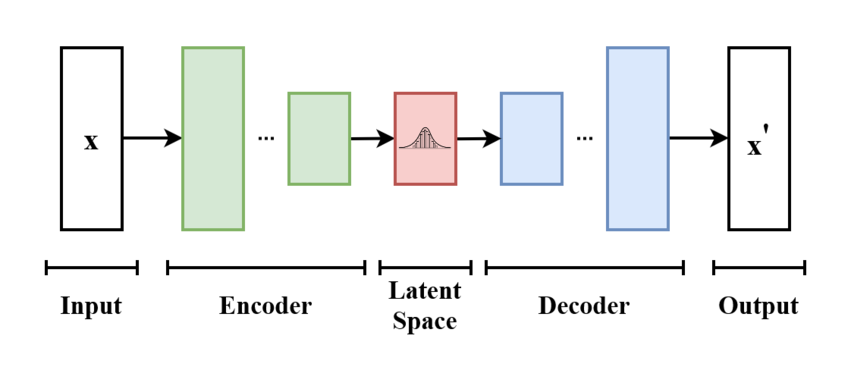
\includegraphics[width=\textwidth]{img/vaewiki.png}
        \caption{VAEs structure \textsuperscript{Source:wikipedia}}
        \label{fig:a}
    \end{subfigure}
    \hfill
        \begin{subfigure}{0.45\textwidth}
    \centering
        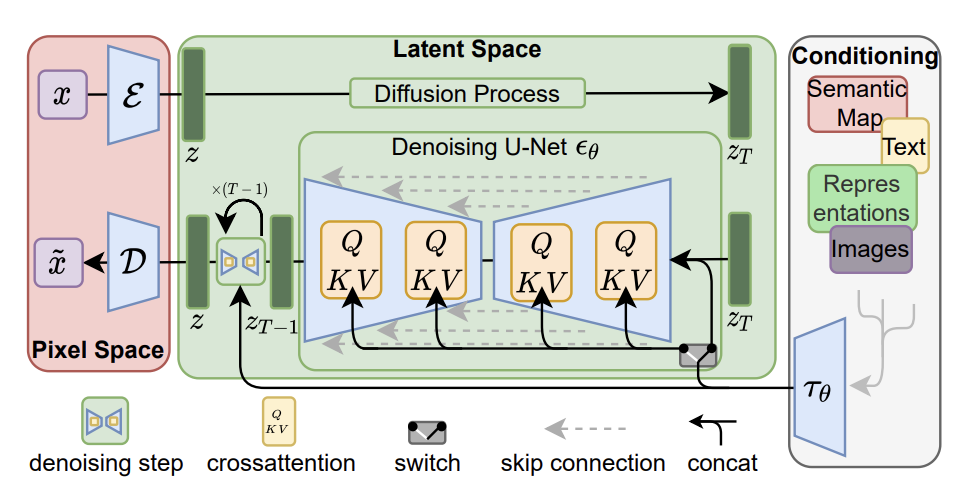
\includegraphics[width=\textwidth]{img/ldm.png}
        \caption{LDMs structure \textsuperscript{Source:\cite{rombach2022highresolutionimagesynthesislatent}}}
        \label{fig:c}
    \end{subfigure}

\end{figure}


\begin{figure}[htp]
    \centering
    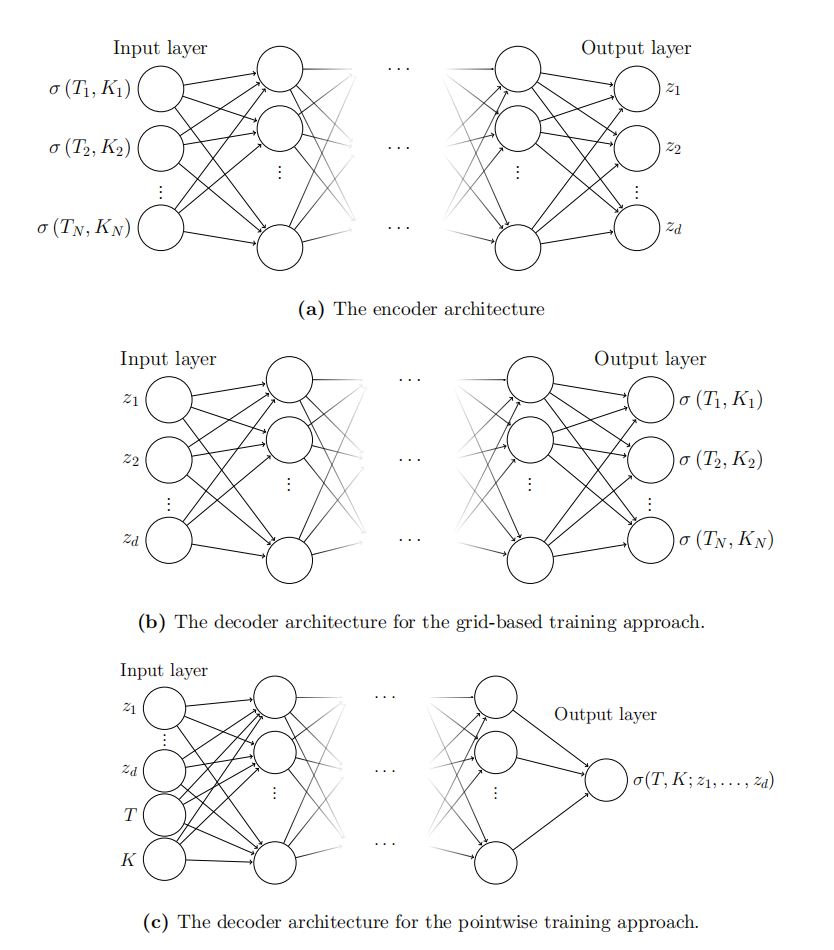
\includegraphics[width=0.6\linewidth]{img/vae_vol.png}
    \caption{Architectures of grid-based and pointwise method}
    \label{fig:b}
\end{figure}


\begin{figure}[!h]
    \centering
    \begin{subfigure}{0.49\textwidth} % 1st subplot
        \centering
        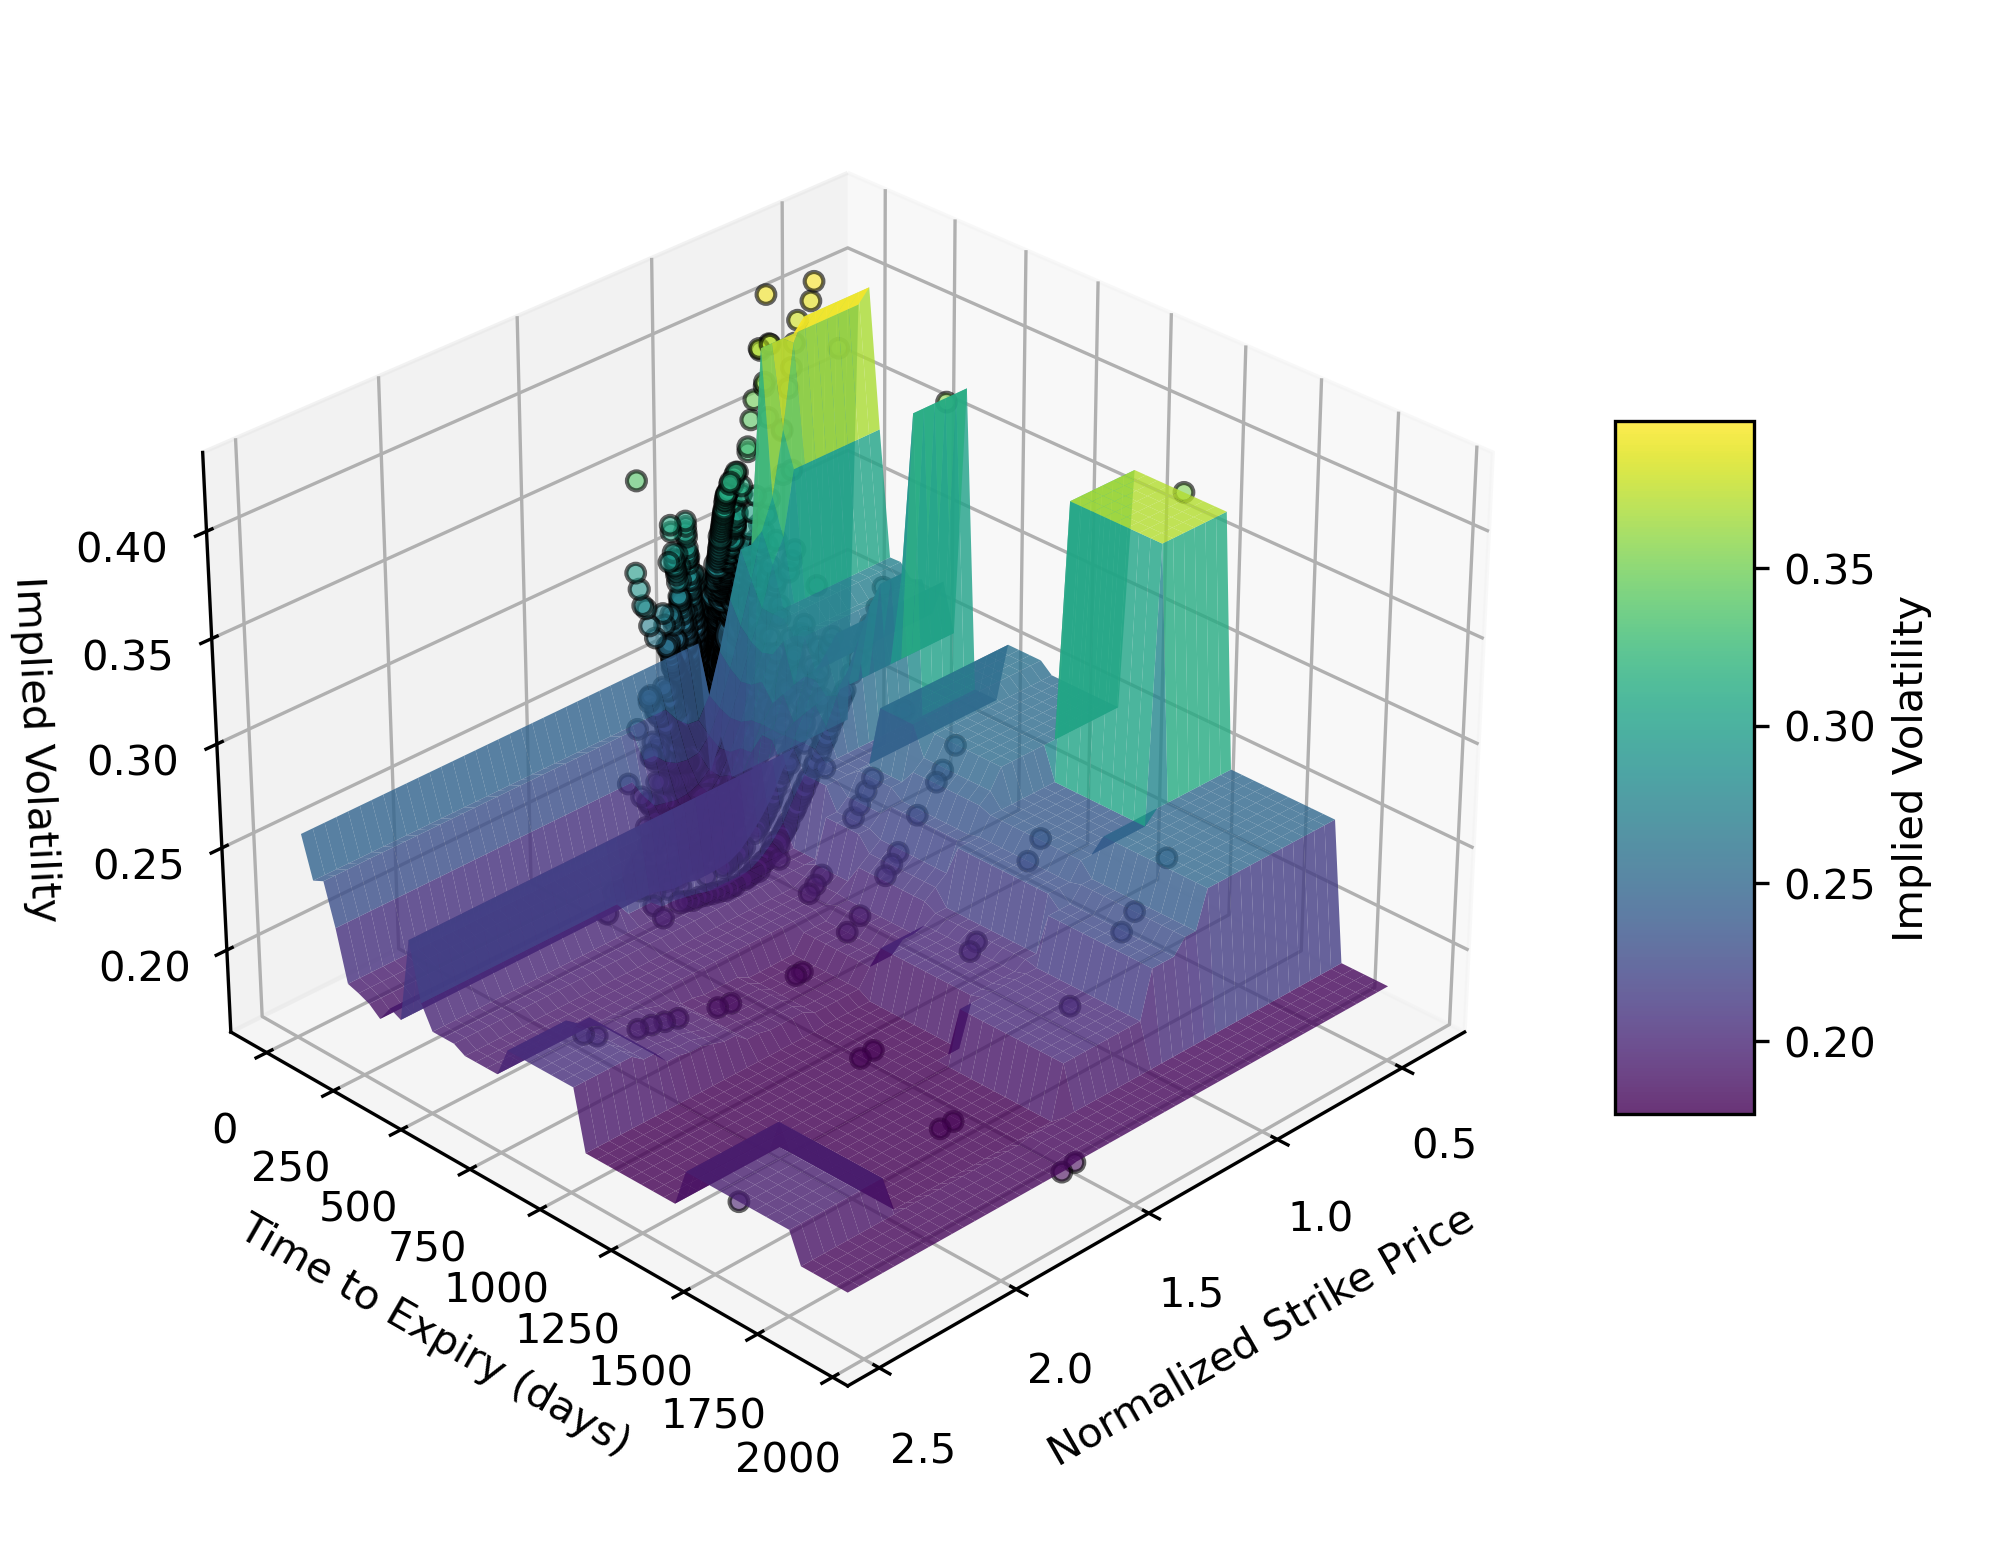
\includegraphics[width=\linewidth]{img/vol_surface_20220923.png}
        \caption{Sep 23, 2022}
    \end{subfigure}
    \hfill
    \begin{subfigure}{0.49\textwidth} % 2nd subplot
        \centering
        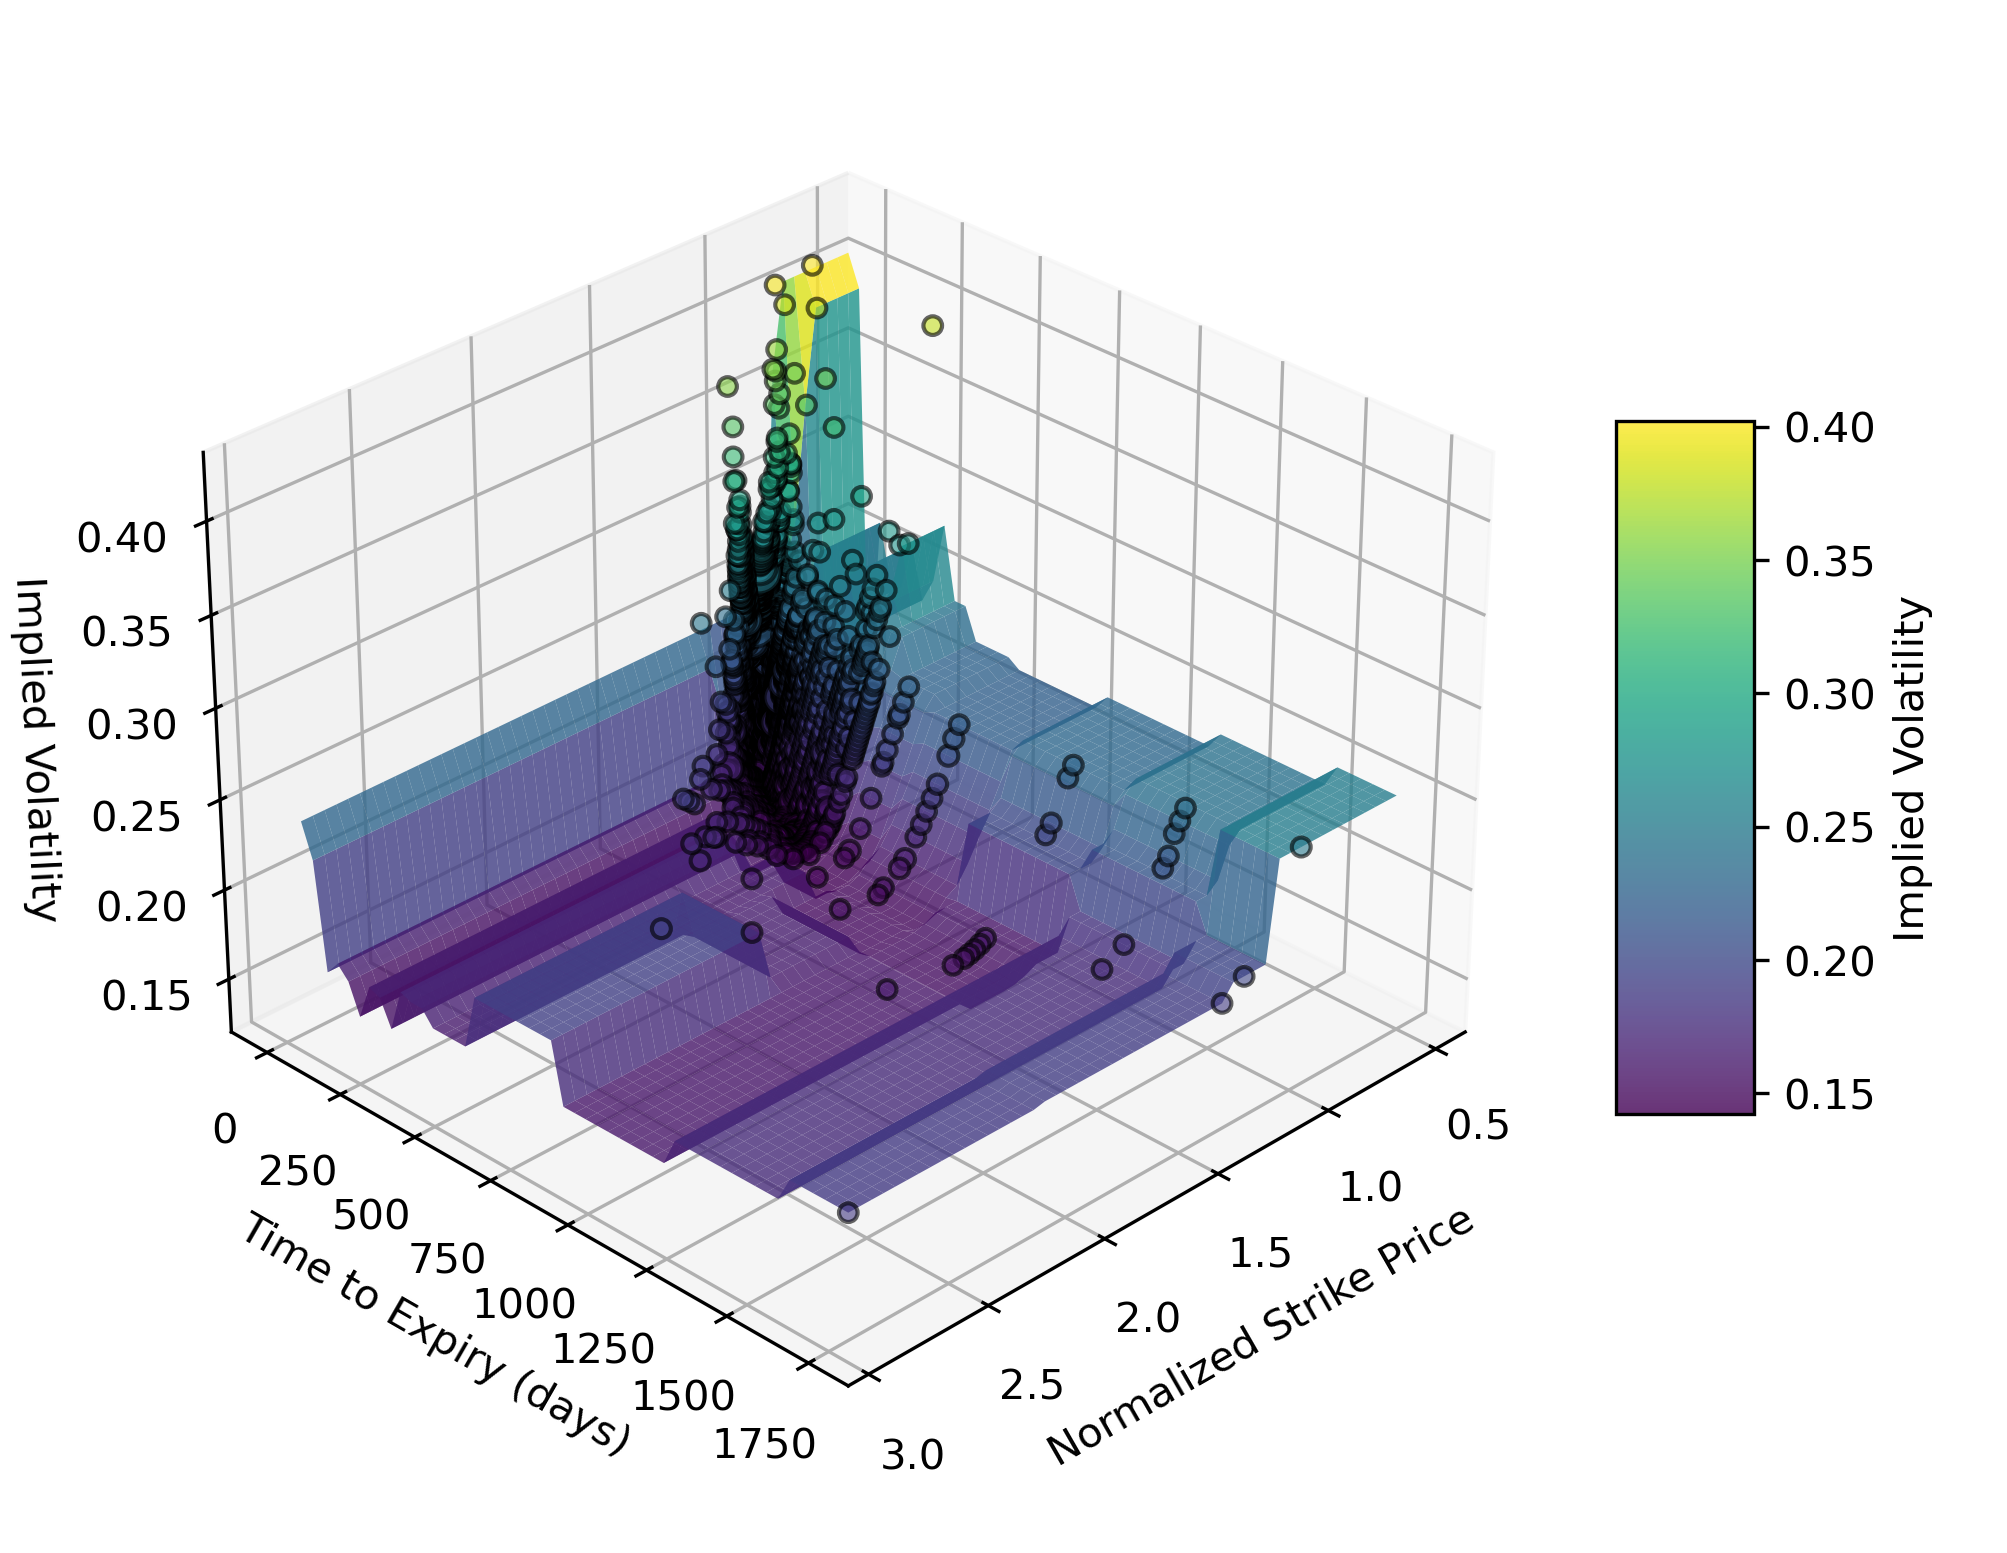
\includegraphics[width=\linewidth]{img/vol_surface_20230310.png}
        \caption{Mar 10, 2023}
    \end{subfigure}

    \vspace{0.5cm} % Vertical space

    \begin{subfigure}{0.49\textwidth} % 3rd subplot
        \centering
        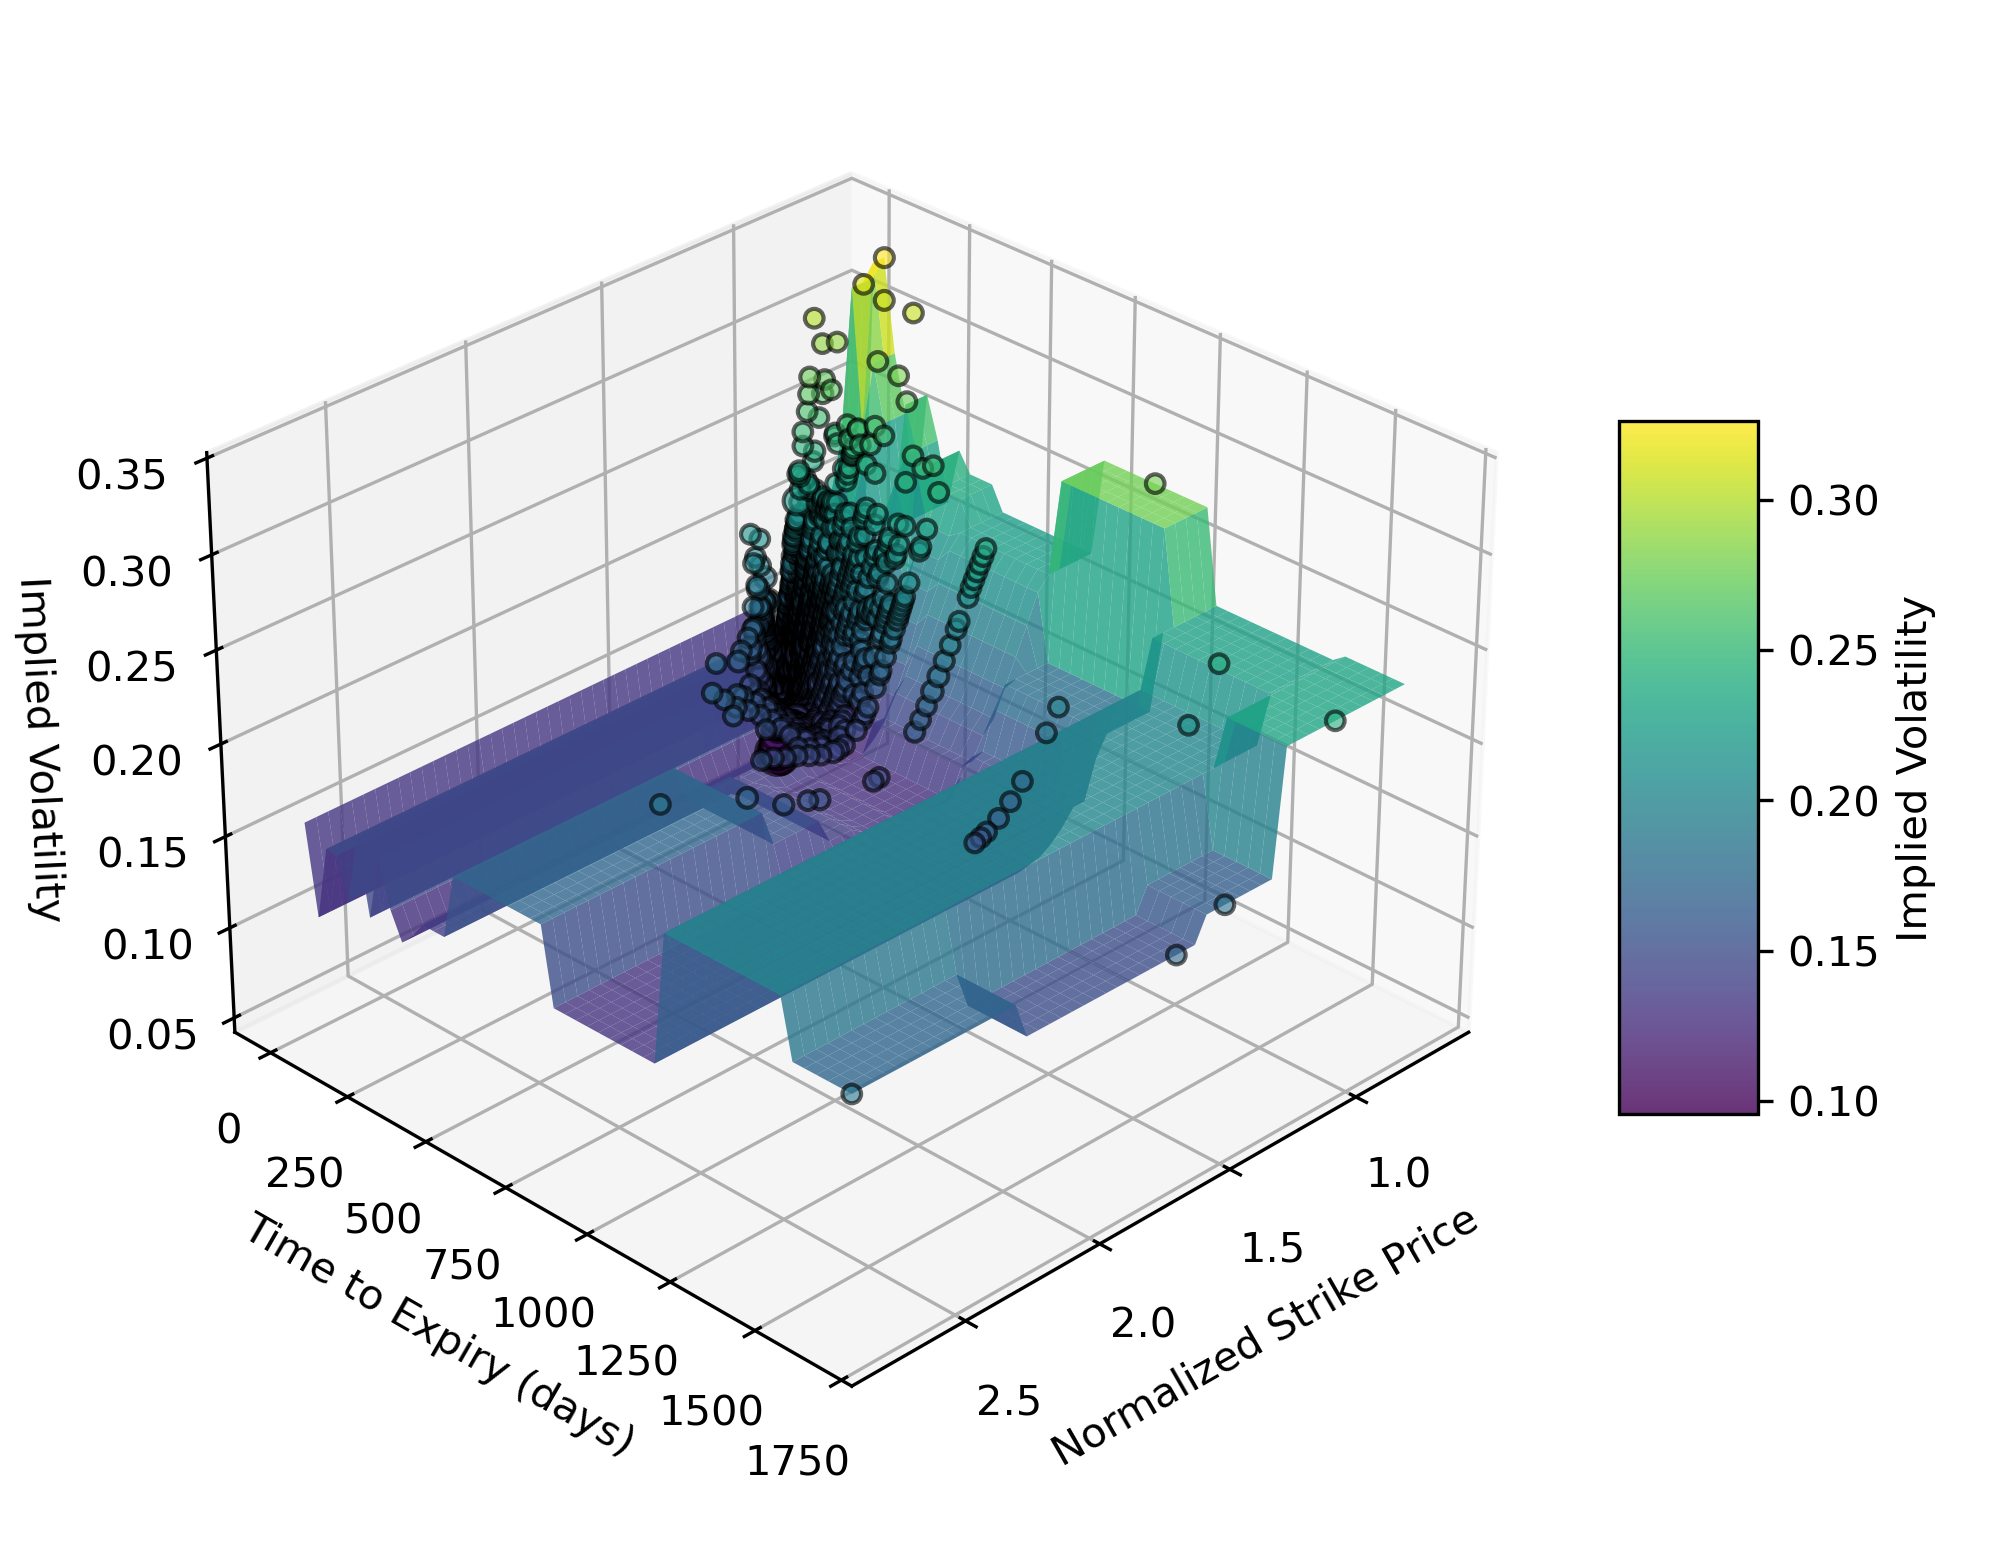
\includegraphics[width=\linewidth]{img/vol_surface_20230602.png}
        \caption{Jun 2, 2023}
    \end{subfigure}
    \hfill
    \begin{subfigure}{0.49\textwidth} % 4th subplot
        \centering
        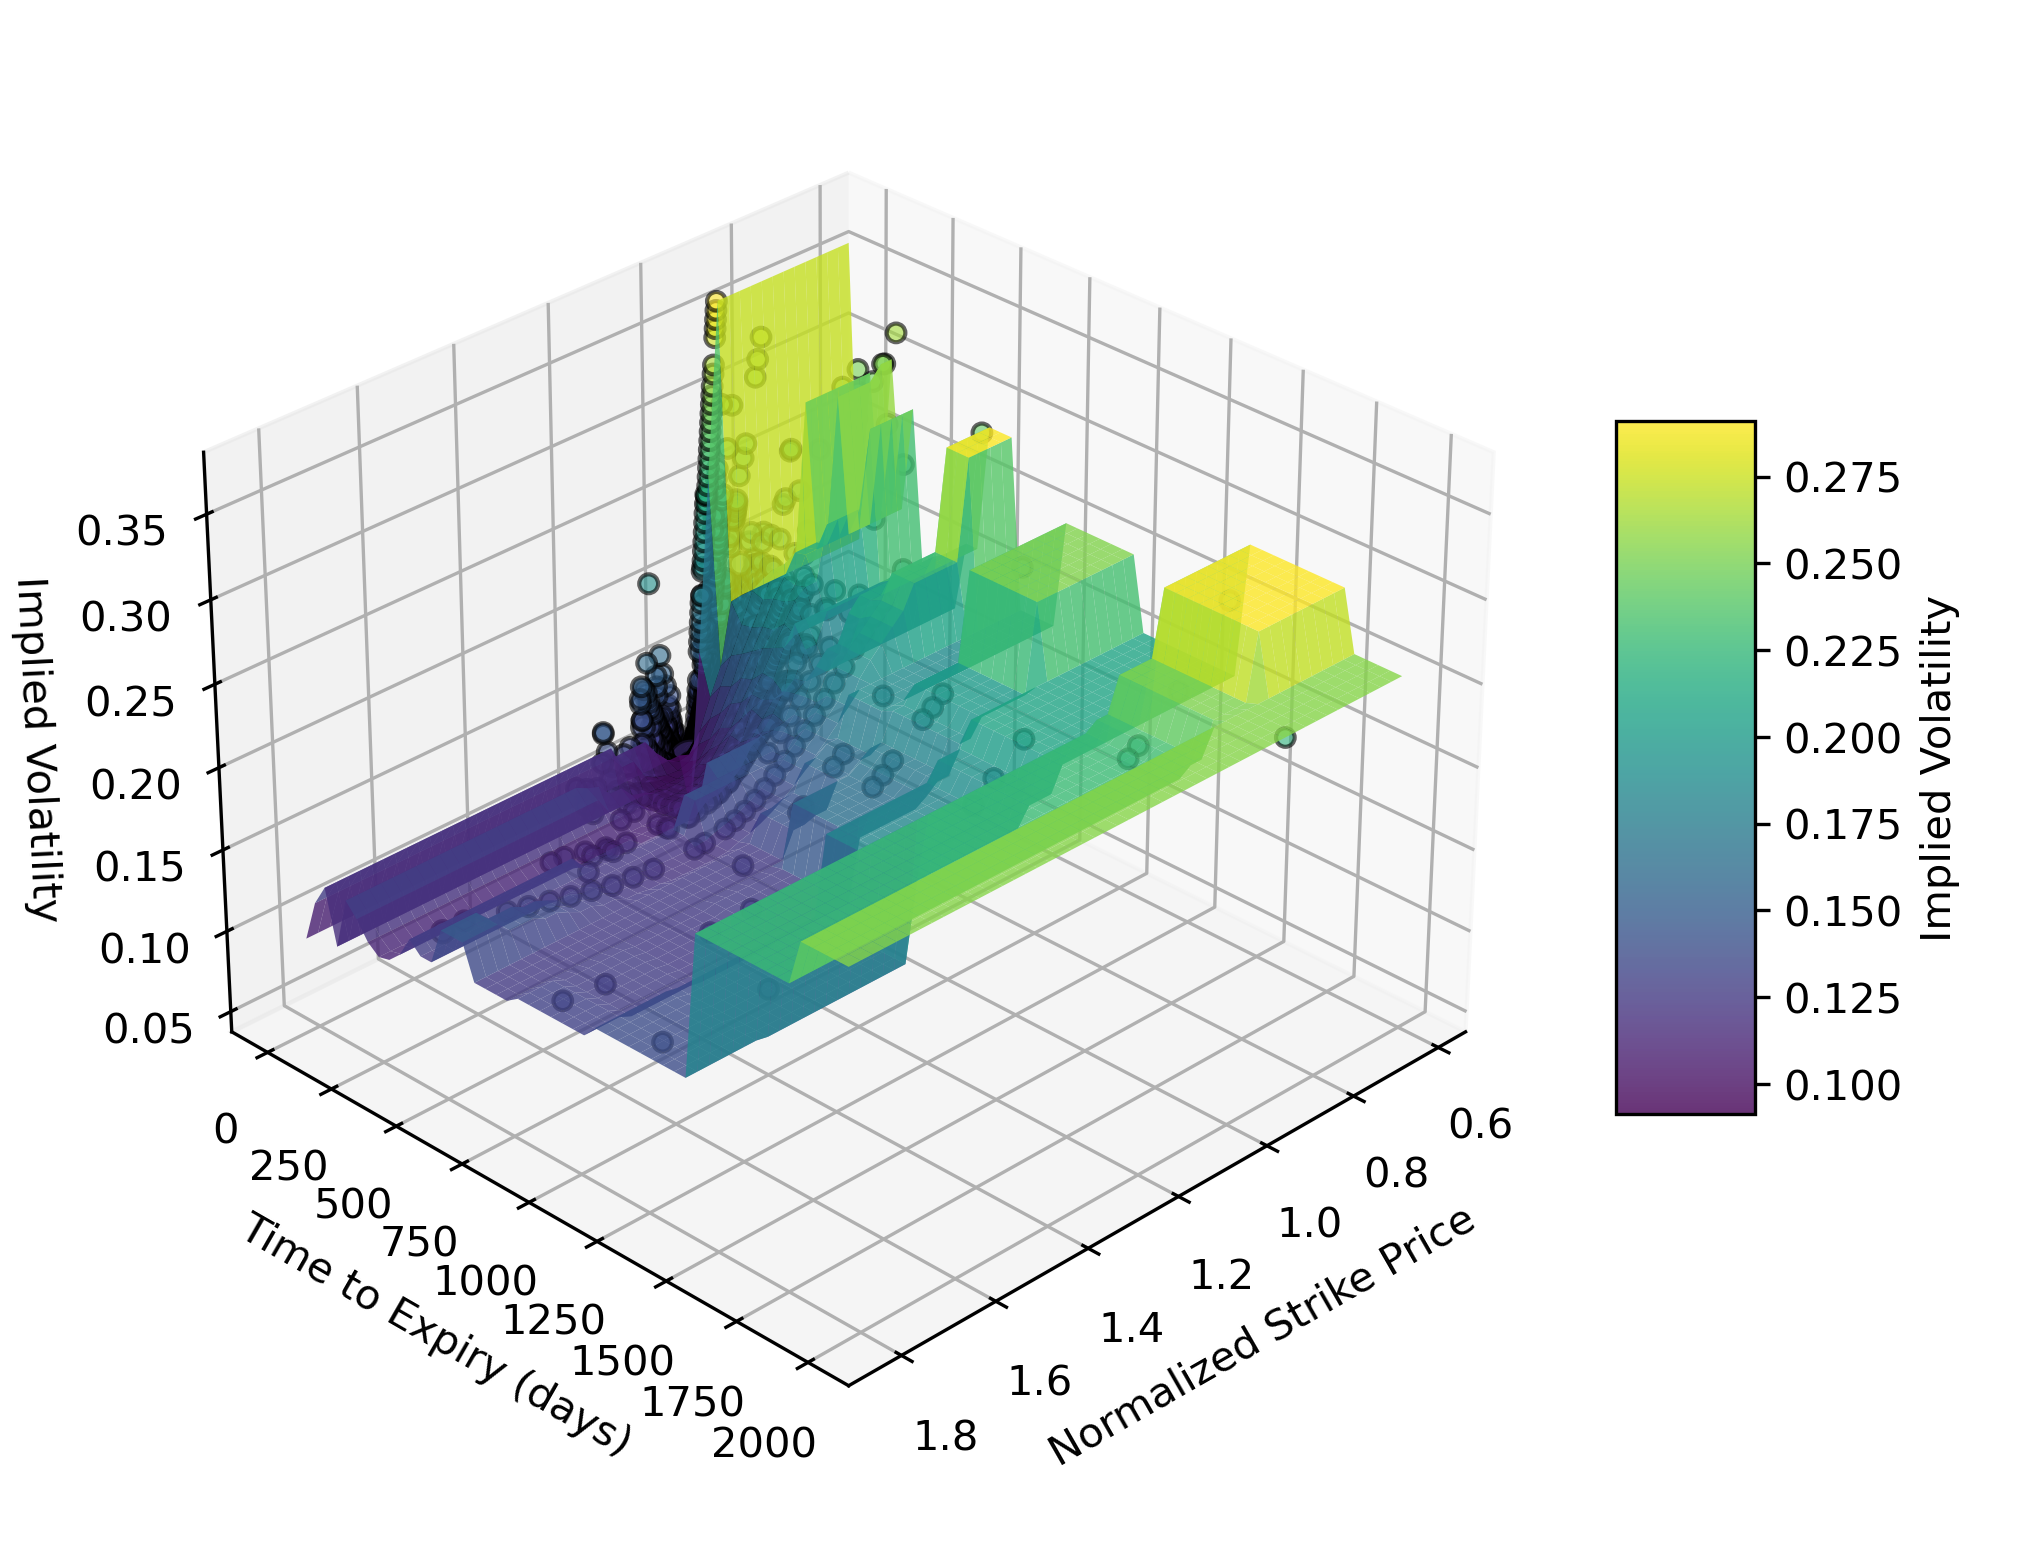
\includegraphics[width=\linewidth]{img/vol_surface_20230630.png}
        \caption{Jun 30, 2023}
    \end{subfigure}
    \caption{Example Volatility Surfaces with the Largest Trading Volume}
    \label{fig:vol_surface}
\end{figure}

\end{document}